\chapter{Model Validation}
\label{chp:MV}

%%%%%%%%%%%%%%%%%%%%%%%%%%%%%%%%%%%%%%%%%%%%%%%%%%%%%%%%%%%%%%%%%%%%%%%

Physical replicas of selected units are constructed and inflated. The deformation is observed and compared with the modelled behaviour as calculated by the FEM software.

\section{FEM}

Units were modelled and manufactured with $\SI{1}{cm}\times \SI{1}{cm}$ sized elements. Only a single unit was manufactured at a time. Constructing a $5\times 5$ grid of the unit is impractical at the current scale. FEM models selected for model validation were adjusted accordingly. Surrounding units were removed. A fixed displacement boundary condition was applied to the bottom left node of the unit.

\section{Mixing and Casting}

The modular mould as described in Section~\ref{ssec:pc} is assembled according to the desired unit layout. Mold Star 15 is mixed and cast as per Section~\ref{ssec:mac}. Figure~\ref{fig:fillmould} shows a filled mould. After the cure time has passed, the unit is removed from the mould and excess material is carefully cut off. 

\begin{figure}[H]
	\centering
	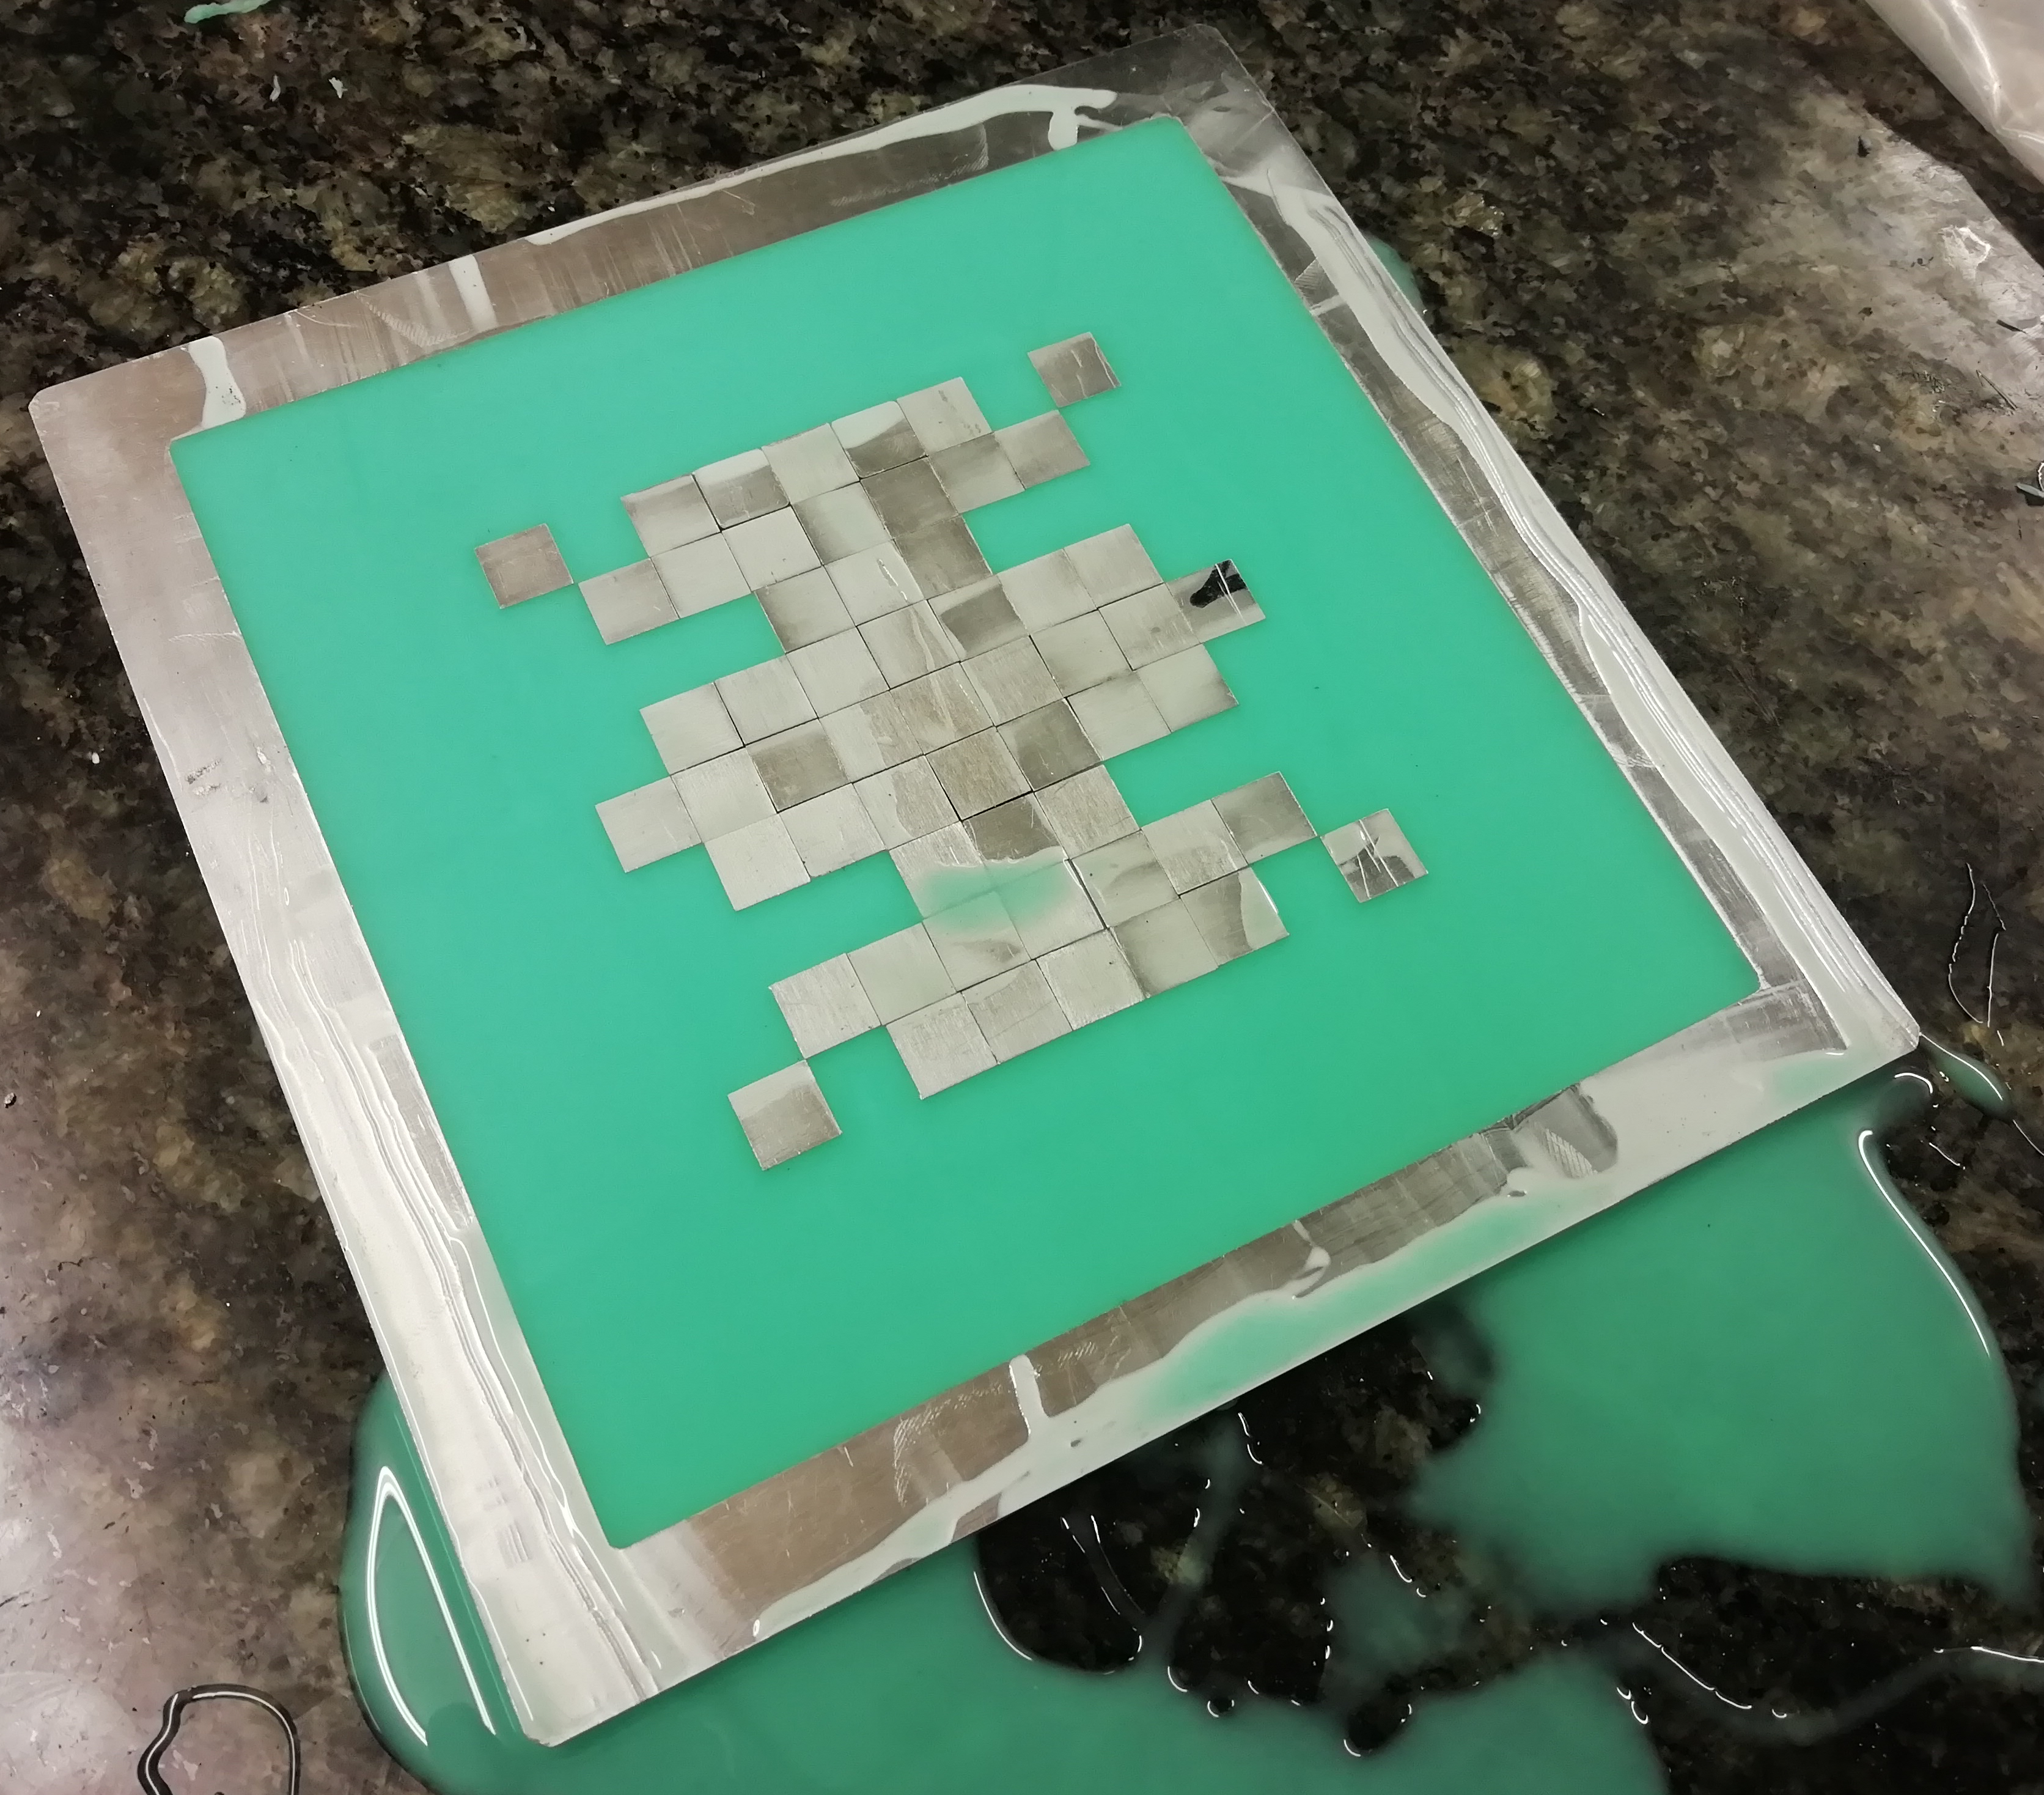
\includegraphics[width=0.5\textwidth]{MouldFilled.png}
	\caption[A filled unit mould]{A unit mould filled with Mold Star 15 before it has cured. Excess material that has been removed is visible around the mould.}
	\label{fig:fillmould}
\end{figure}

\section{Experimental Setup}

The experimental setup as described in Section~\ref{ssec:pc} is constructed. Figure~\ref{fig:expempty} shows the experimental setup with no unit in place.

\begin{figure}[H]
	\centering
	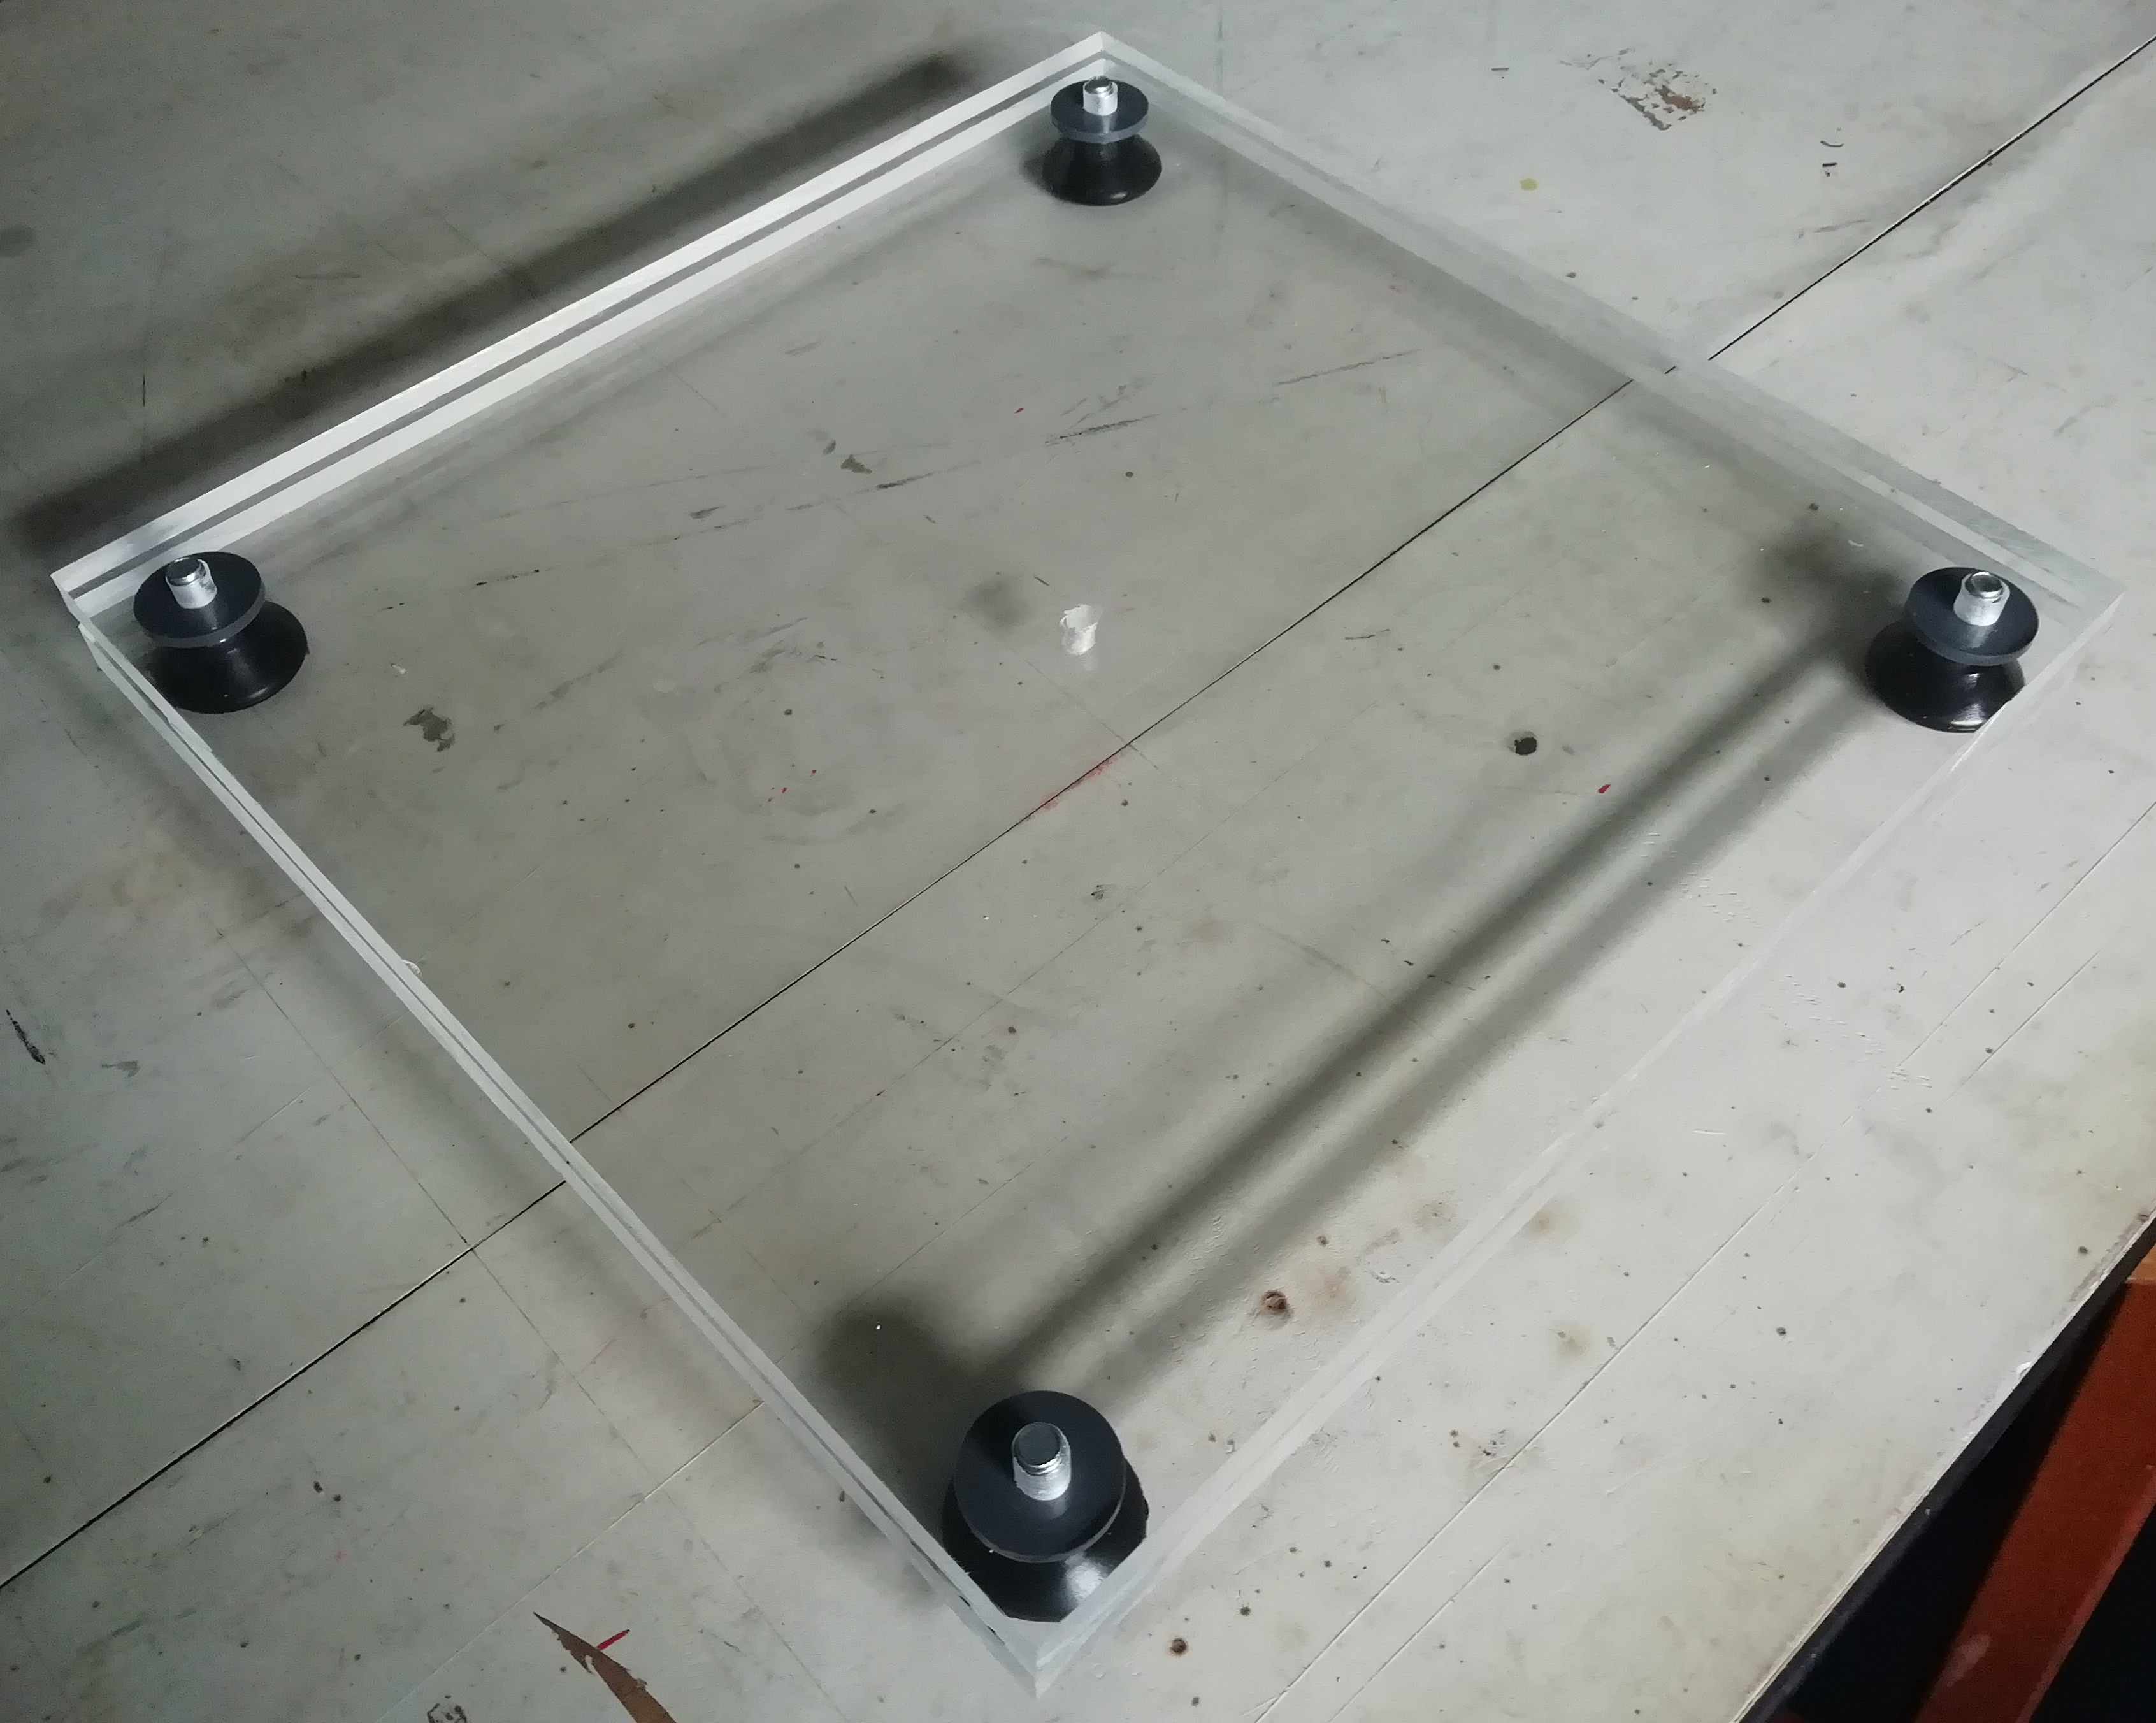
\includegraphics[width=0.5\textwidth]{rig_empty.png}
	\caption[The experimental setup without a unit]{The experimental setup with no unit in place and the pressure hose unconnected}
	\label{fig:expempty}
\end{figure}

The pressure hose is inserted into the hole in the bottom plate. A sealant is applied to prevent air leakage at the point of entry of the pressure hose.

\section{Results}

Three units were selected for model validation.

\subsection{Unit 1}

The first unit selected is grid\_36\_d68df4e04590e068b46c0e75dcdf5818. This unit was selected as a random control unit. This unit does not perform well according to any specific unit deformation case. This unit has complex internal geometry that may deform in unusual ways. Cavities exist which are potentially inaccessible from the undeformed state, but become accessible as the unit inflates. An additional cavity exists which is not accessible with the experimental setup. This was replicated in the FEM model. The FEM model with boundary conditions is illustrated in Figure~\ref{fig:unit1bc}. The physical model is illustrated in Figure~\ref{fig:unit1mod}.

\begin{figure}[H]
	\centering
	\begin{subfigure}[t]{0.5\textwidth}
		\includegraphics[width=\textwidth]{unit1bc.png}
		\caption{FEM validation model with applied boundary conditions}
		\label{fig:unit1bc}
	\end{subfigure}
	\hfill
	\begin{subfigure}[t]{0.4\textwidth}
		\centering
		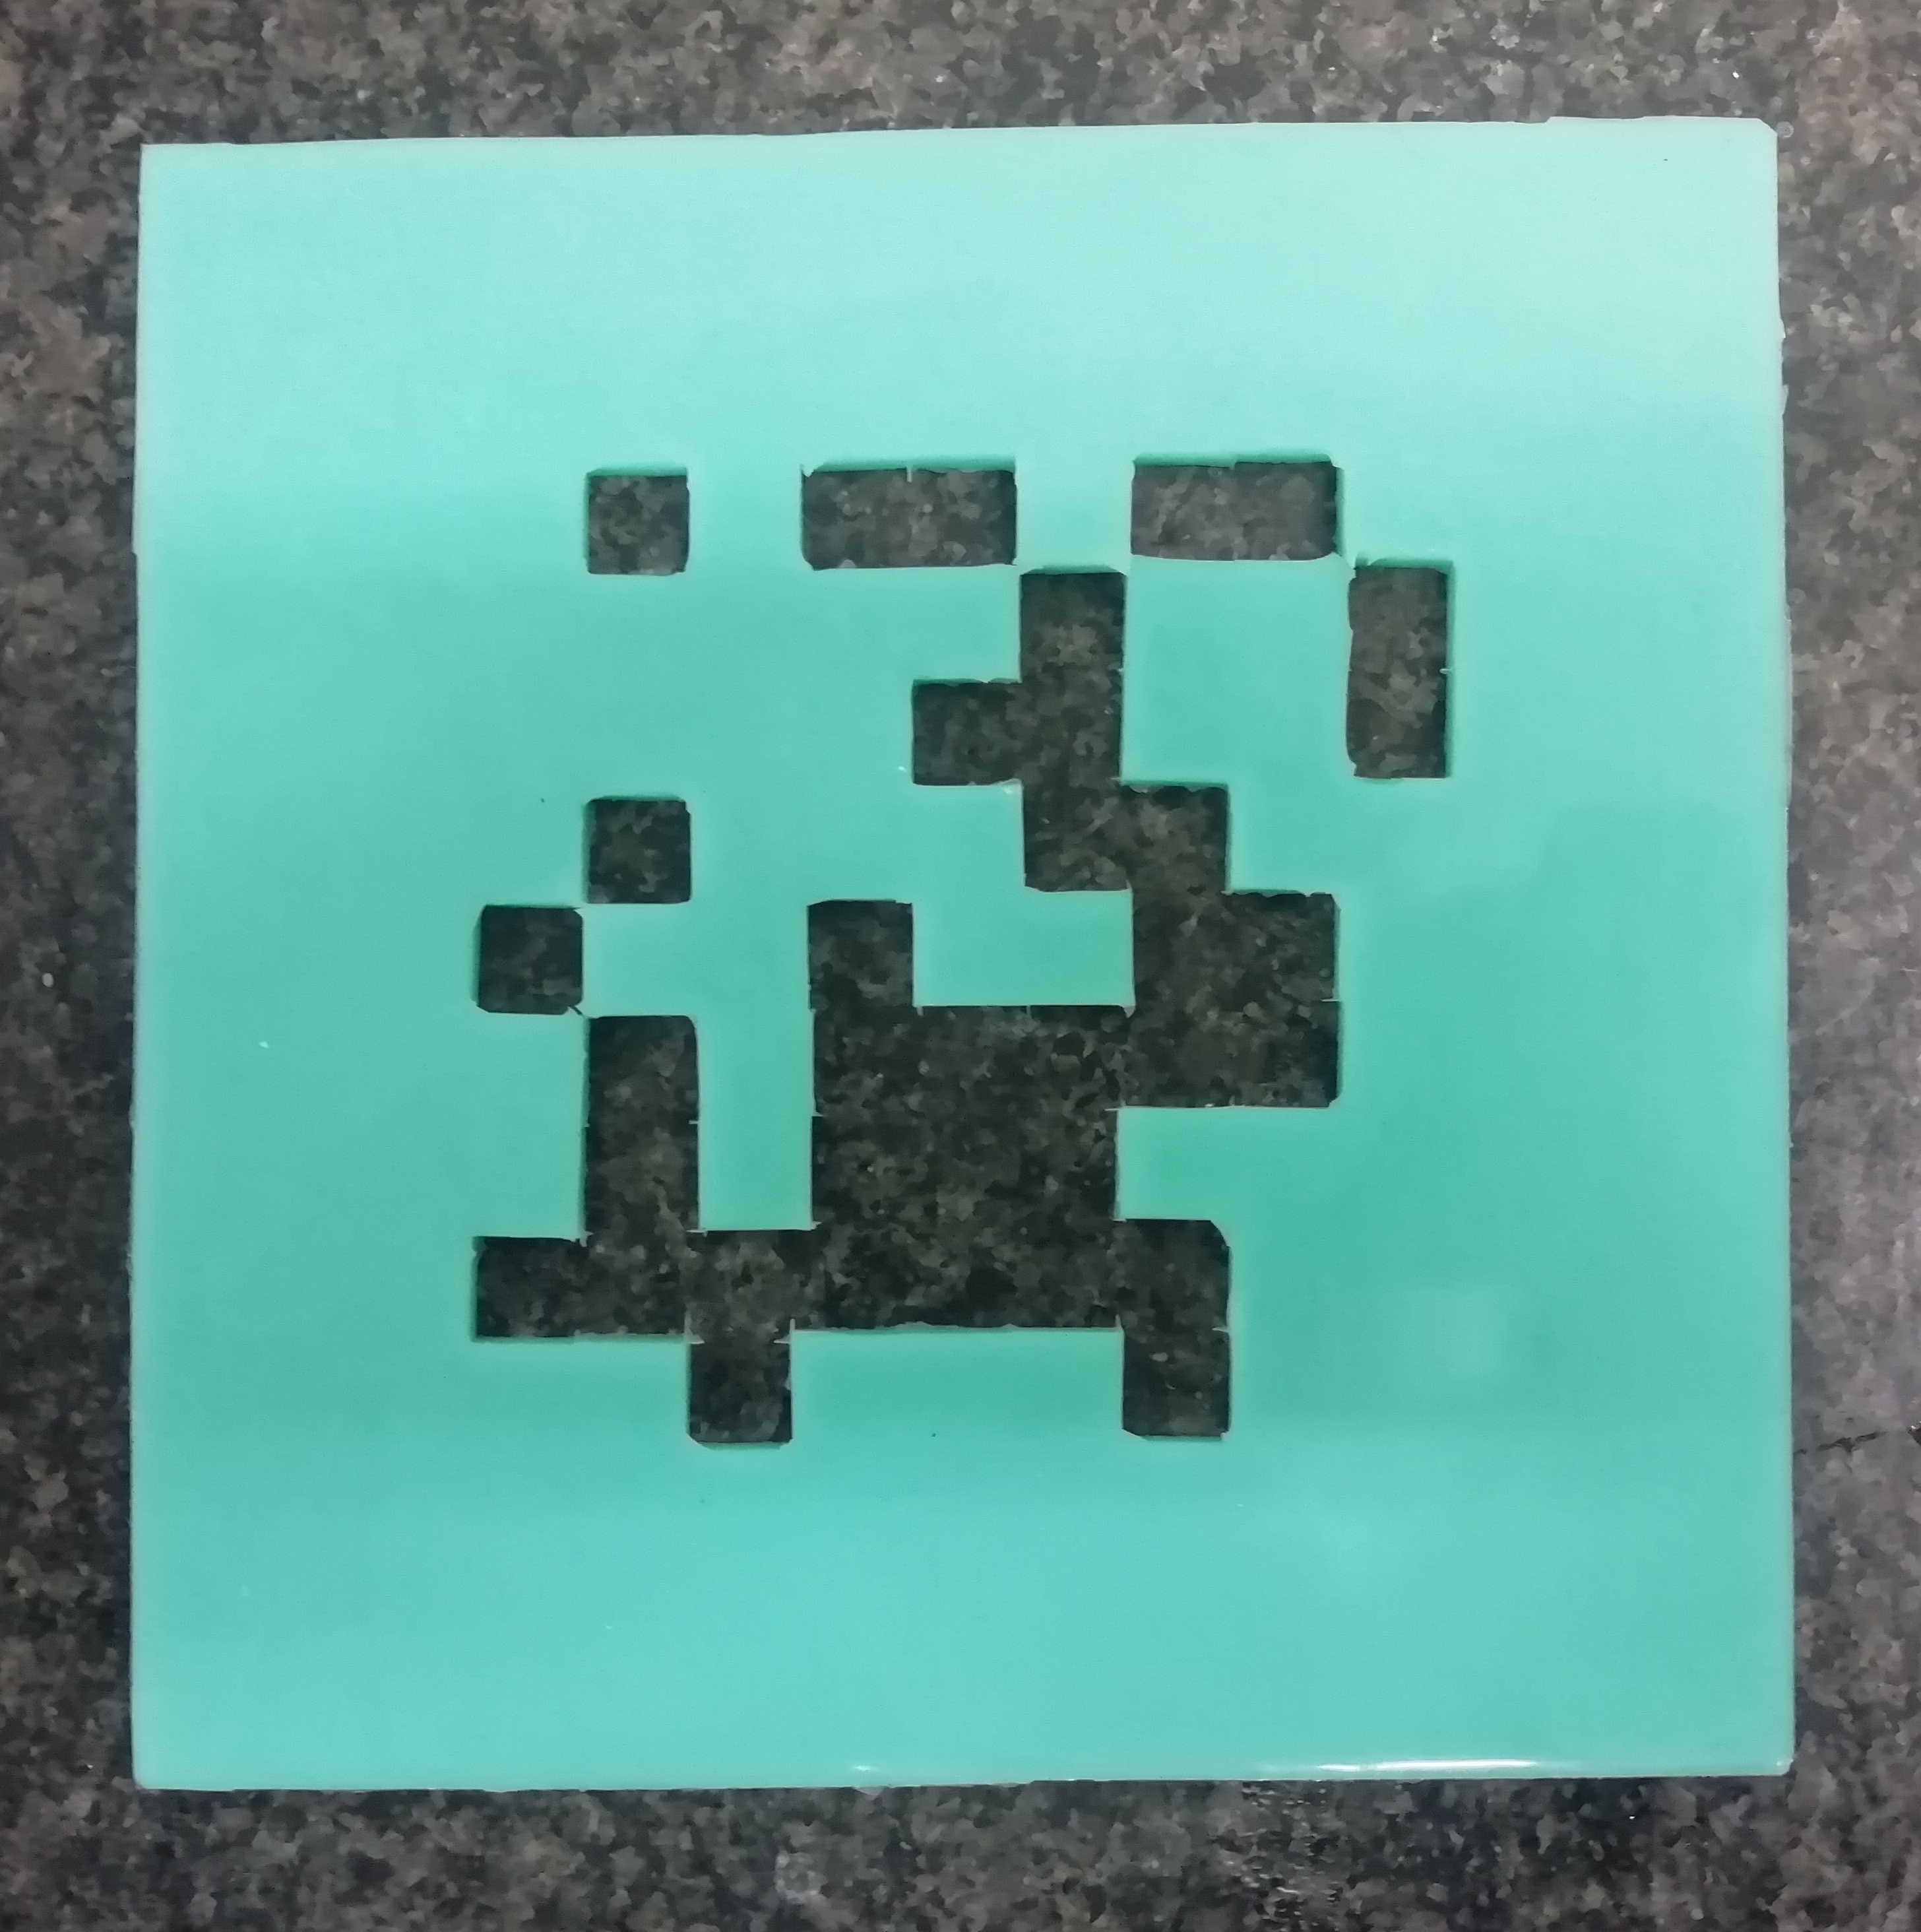
\includegraphics[width=\textwidth]{unit1mod.png}
		\caption{Physical validation model}
		\label{fig:unit1mod}
	\end{subfigure}
	\caption[FEM and physical models of unit 1]{grid\_36\_d68df4e04590e068b46c0e75dcdf5818 FEM and physical validation models}
	\label{fig:unit1}
\end{figure}

Figure~\ref{fig:unit1def} shows comparisons between the FEM model and the physical model as the internal pressure is increased. Figure~\ref{fig:unit1over} illustrates an overlay of the FEM model deformation with the physical model's deformation. The FEM deformation is taken from step 2 of the simulation. The physical deformation is the final deformation.

\begin{figure}[H]
	\centering
	\begin{subfigure}[c]{\textwidth}
		\centering
		\includegraphics[width=\textwidth]{unit1deffem.png}
		\caption{FEM model deformation as internal pressure is increased. Steps 0-5 of the simulation are shown from left to right.}
	\end{subfigure}
	\hfill
	\begin{subfigure}[c]{\textwidth}
		\centering
		\includegraphics[width=\textwidth]{unit1defmod.png}
		\caption{Physical model deformation as internal pressure is increased}
	\end{subfigure}
	\caption[Comparison between FEM and physical models of unit 1]{Comparison between the deformation of the FEM model and physical model of grid\_36\_d68df4e04590e068b46c0e75dcdf5818 as the internal pressure is increased}
	\label{fig:unit1def}
\end{figure}

\begin{figure}[H]
	\centering
	\includegraphics[width=0.8\textwidth]{unit1defover.png}
	\caption[Physical model of unit 1 overlayed with FEM model]{grid\_36\_d68df4e04590e068b46c0e75dcdf5818 physical model overlayed with FEM model at step 2 of simulation}
	\label{fig:unit1over}
\end{figure}

\subsection{Unit 2}

The second unit selected is grid\_57\_292a241d90d8d6b4753d110deca32360. This unit was selected as a linearly extending unit. This unit performs well according to the uniaxial deformation case. Cavities exist which are potentially inaccessible from the undeformed state, but become accessible as the unit inflates. The FEM model with boundary conditions is illustrated in Figure~\ref{fig:unit2bc}. The physical model is illustrated in Figure~\ref{fig:unit2mod}.

\begin{figure}[H]
	\centering
	\begin{subfigure}[t]{0.5\textwidth}
		\includegraphics[width=\textwidth]{unit2bc.png}
		\caption{FEM validation model with applied boundary conditions}
		\label{fig:unit2bc}
	\end{subfigure}
	\hfill
	\begin{subfigure}[t]{0.4\textwidth}
		\centering
		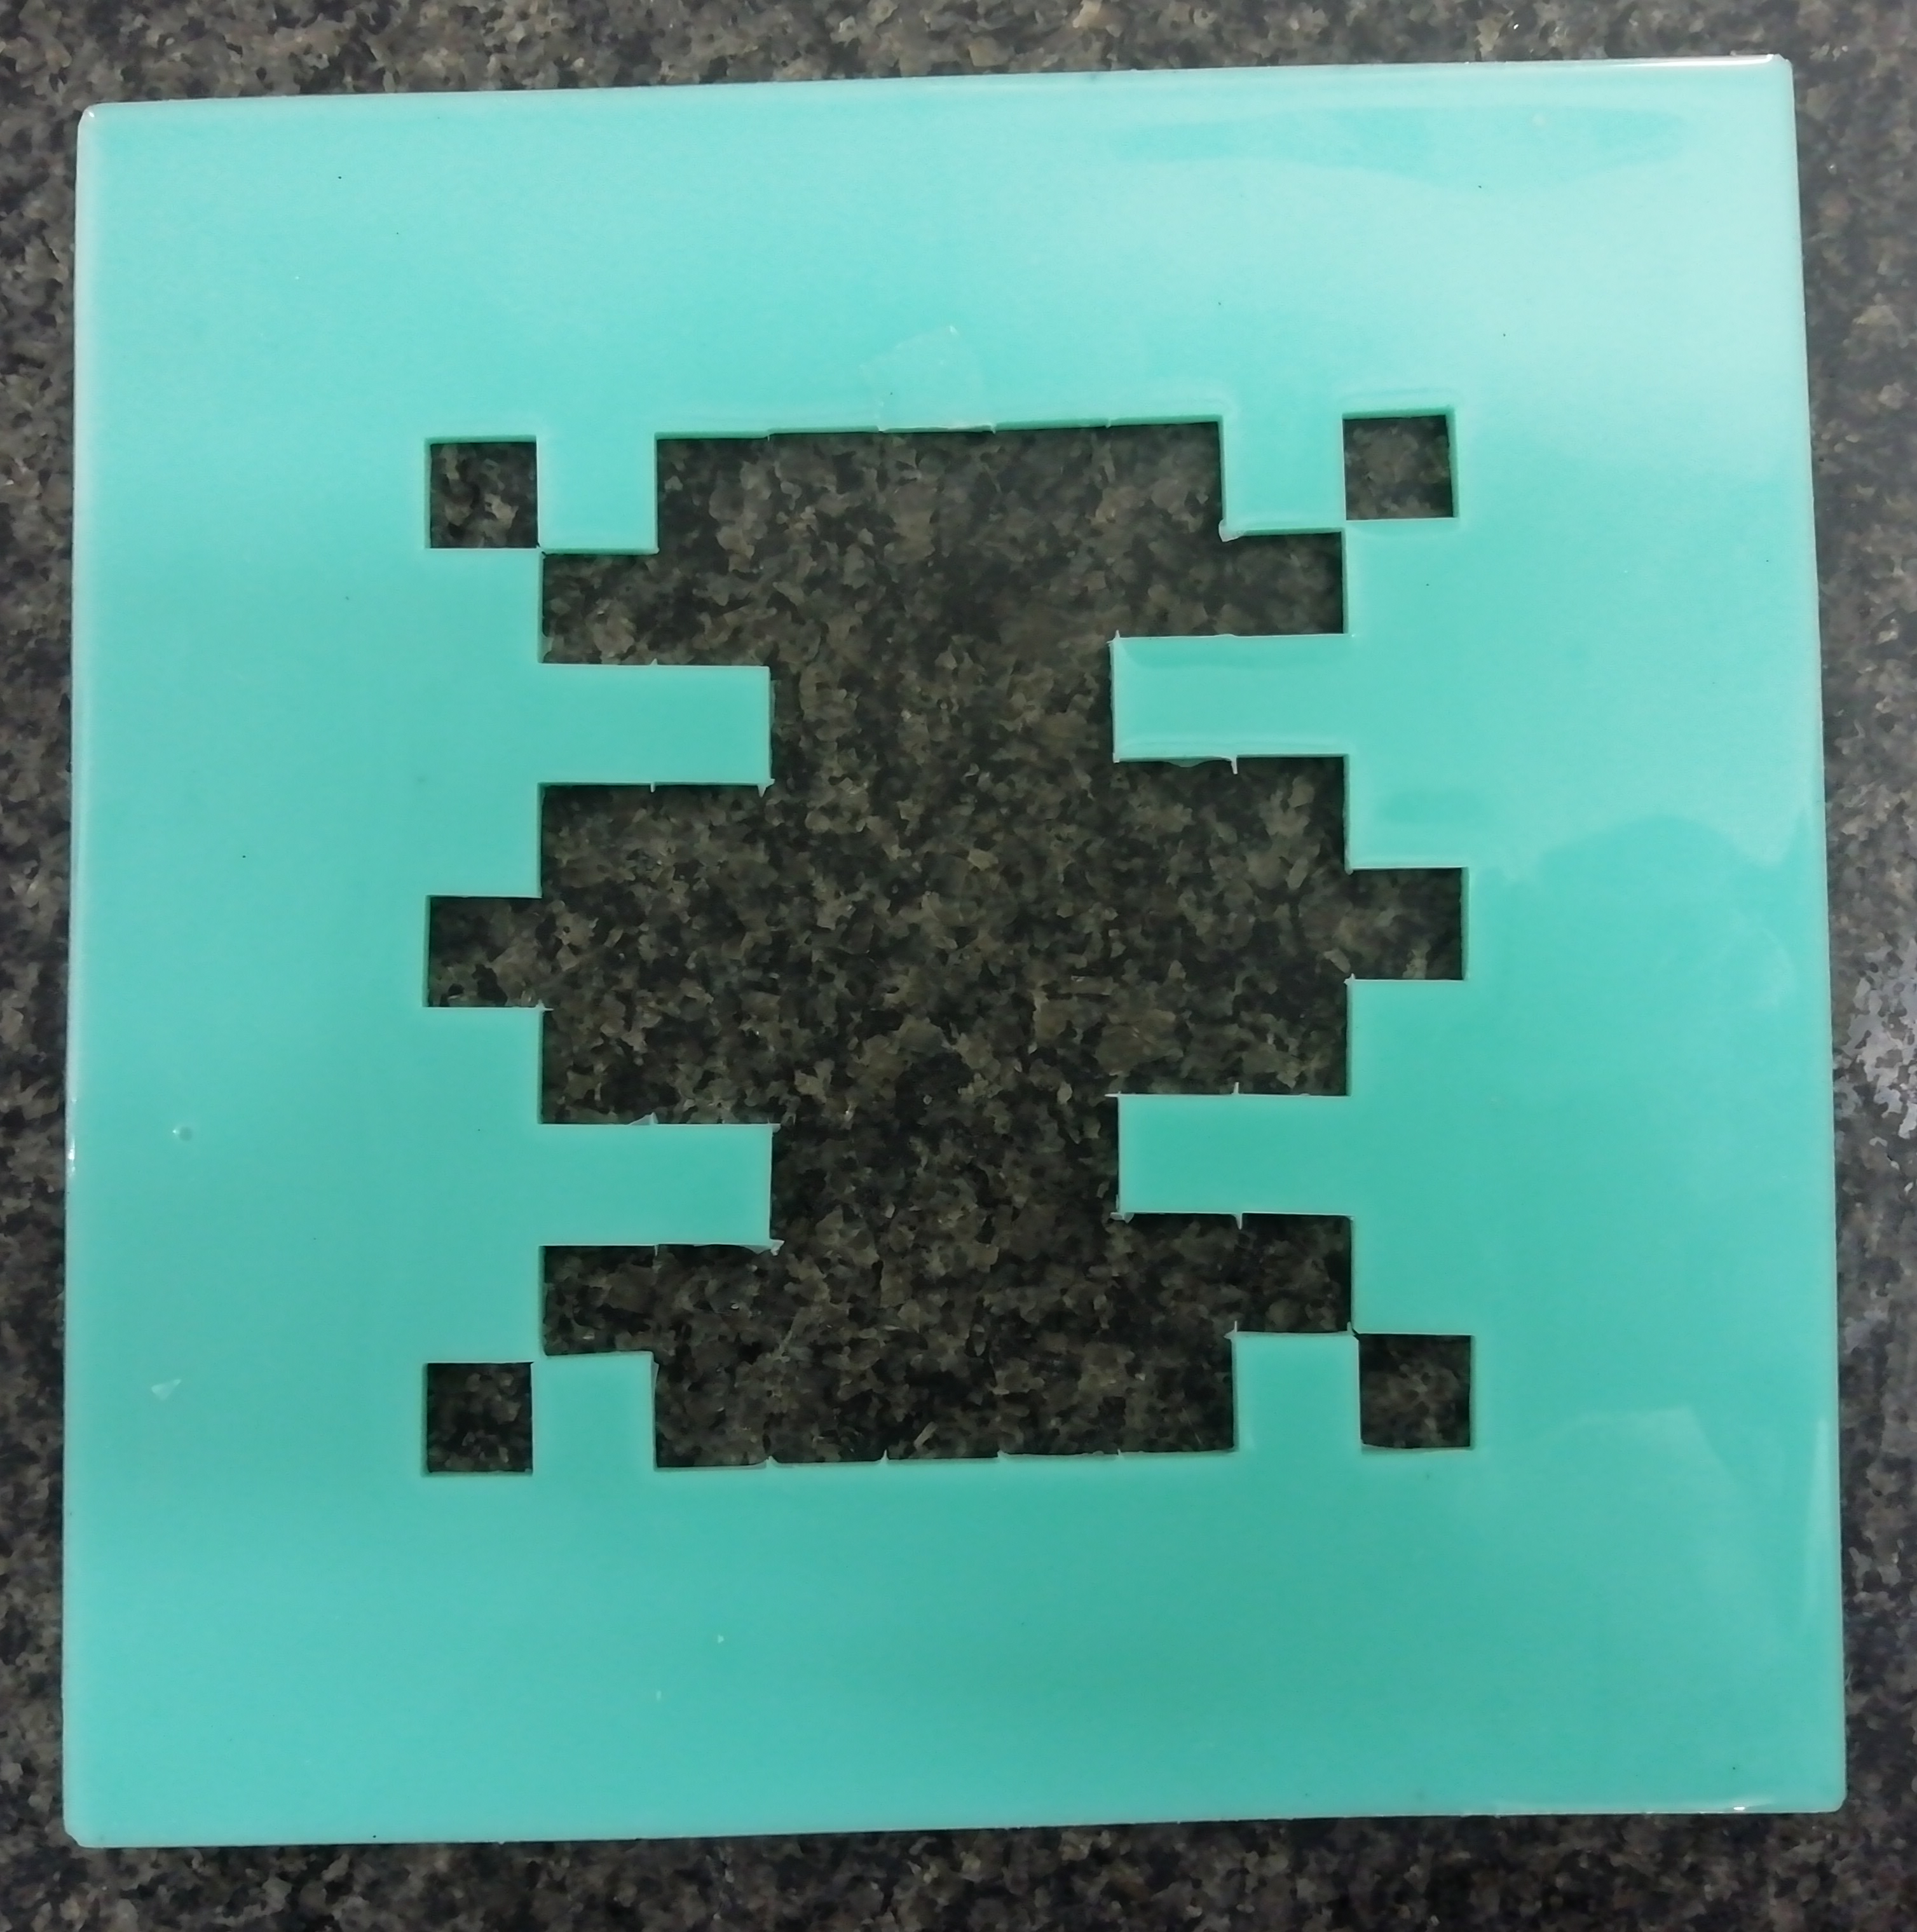
\includegraphics[width=\textwidth]{unit2mod.png}
		\caption{Physical validation model}
		\label{fig:unit2mod}
	\end{subfigure}
	\caption[FEM and physical models of unit 2]{grid\_57\_292a241d90d8d6b4753d110deca32360 FEM and physical validation models}
	\label{fig:unit2}
\end{figure}

Figure~\ref{fig:unit2def} shows comparisons between the FEM model and the physical model as the internal pressure is increased. Figure~\ref{fig:unit2over} illustrates an overlay of the FEM model deformation with the physical model's deformation. The FEM deformation is taken from step 3 of the simulation. The physical deformation is the final deformation.

\begin{figure}[H]
	\centering
	\begin{subfigure}[c]{\textwidth}
		\centering
		\includegraphics[width=\textwidth]{unit2deffem.png}
		\caption{FEM model deformation as internal pressure is increased. Steps 0-5 of the simulation are shown from left to right.}
	\end{subfigure}
	\hfill
	\begin{subfigure}[c]{\textwidth}
		\centering
		\includegraphics[width=\textwidth]{unit2defmod.png}
		\caption{Physical model deformation as internal pressure is increased}
	\end{subfigure}
	\caption[Comparison between FEM and physical models of unit 2]{Comparison between the deformation of the FEM model and physical model of grid\_57\_292a241d90d8d6b4753d110deca32360 as the internal pressure is increased}
	\label{fig:unit2def}
\end{figure}

\begin{figure}[H]
	\centering
	\includegraphics[width=0.8\textwidth]{unit2defover.png}
	\caption[Physical model of unit 2 overlayed with FEM model]{grid\_57\_292a241d90d8d6b4753d110deca32360 physical model overlayed with FEM model at step 4 of simulation}
	\label{fig:unit2over}
\end{figure}

\subsection{Unit 3}

The third unit selected is grid\_50\_9a02e87afe77b71561f73745d87b35bd. This unit was selected as a linearly extending unit. This unit performs well according to the uniaxial deformation case when surrounded by identical units, but performs poorly when on its own. The FEM model with boundary conditions is illustrated in Figure~\ref{fig:unit3bc}. The physical model is illustrated in Figure~\ref{fig:unit3mod}.

\begin{figure}[H]
	\centering
	\begin{subfigure}[t]{0.5\textwidth}
		\includegraphics[width=\textwidth]{unit3bc.png}
		\caption{FEM validation model with applied boundary conditions}
		\label{fig:unit3bc}
	\end{subfigure}
	\hfill
	\begin{subfigure}[t]{0.4\textwidth}
		\centering
		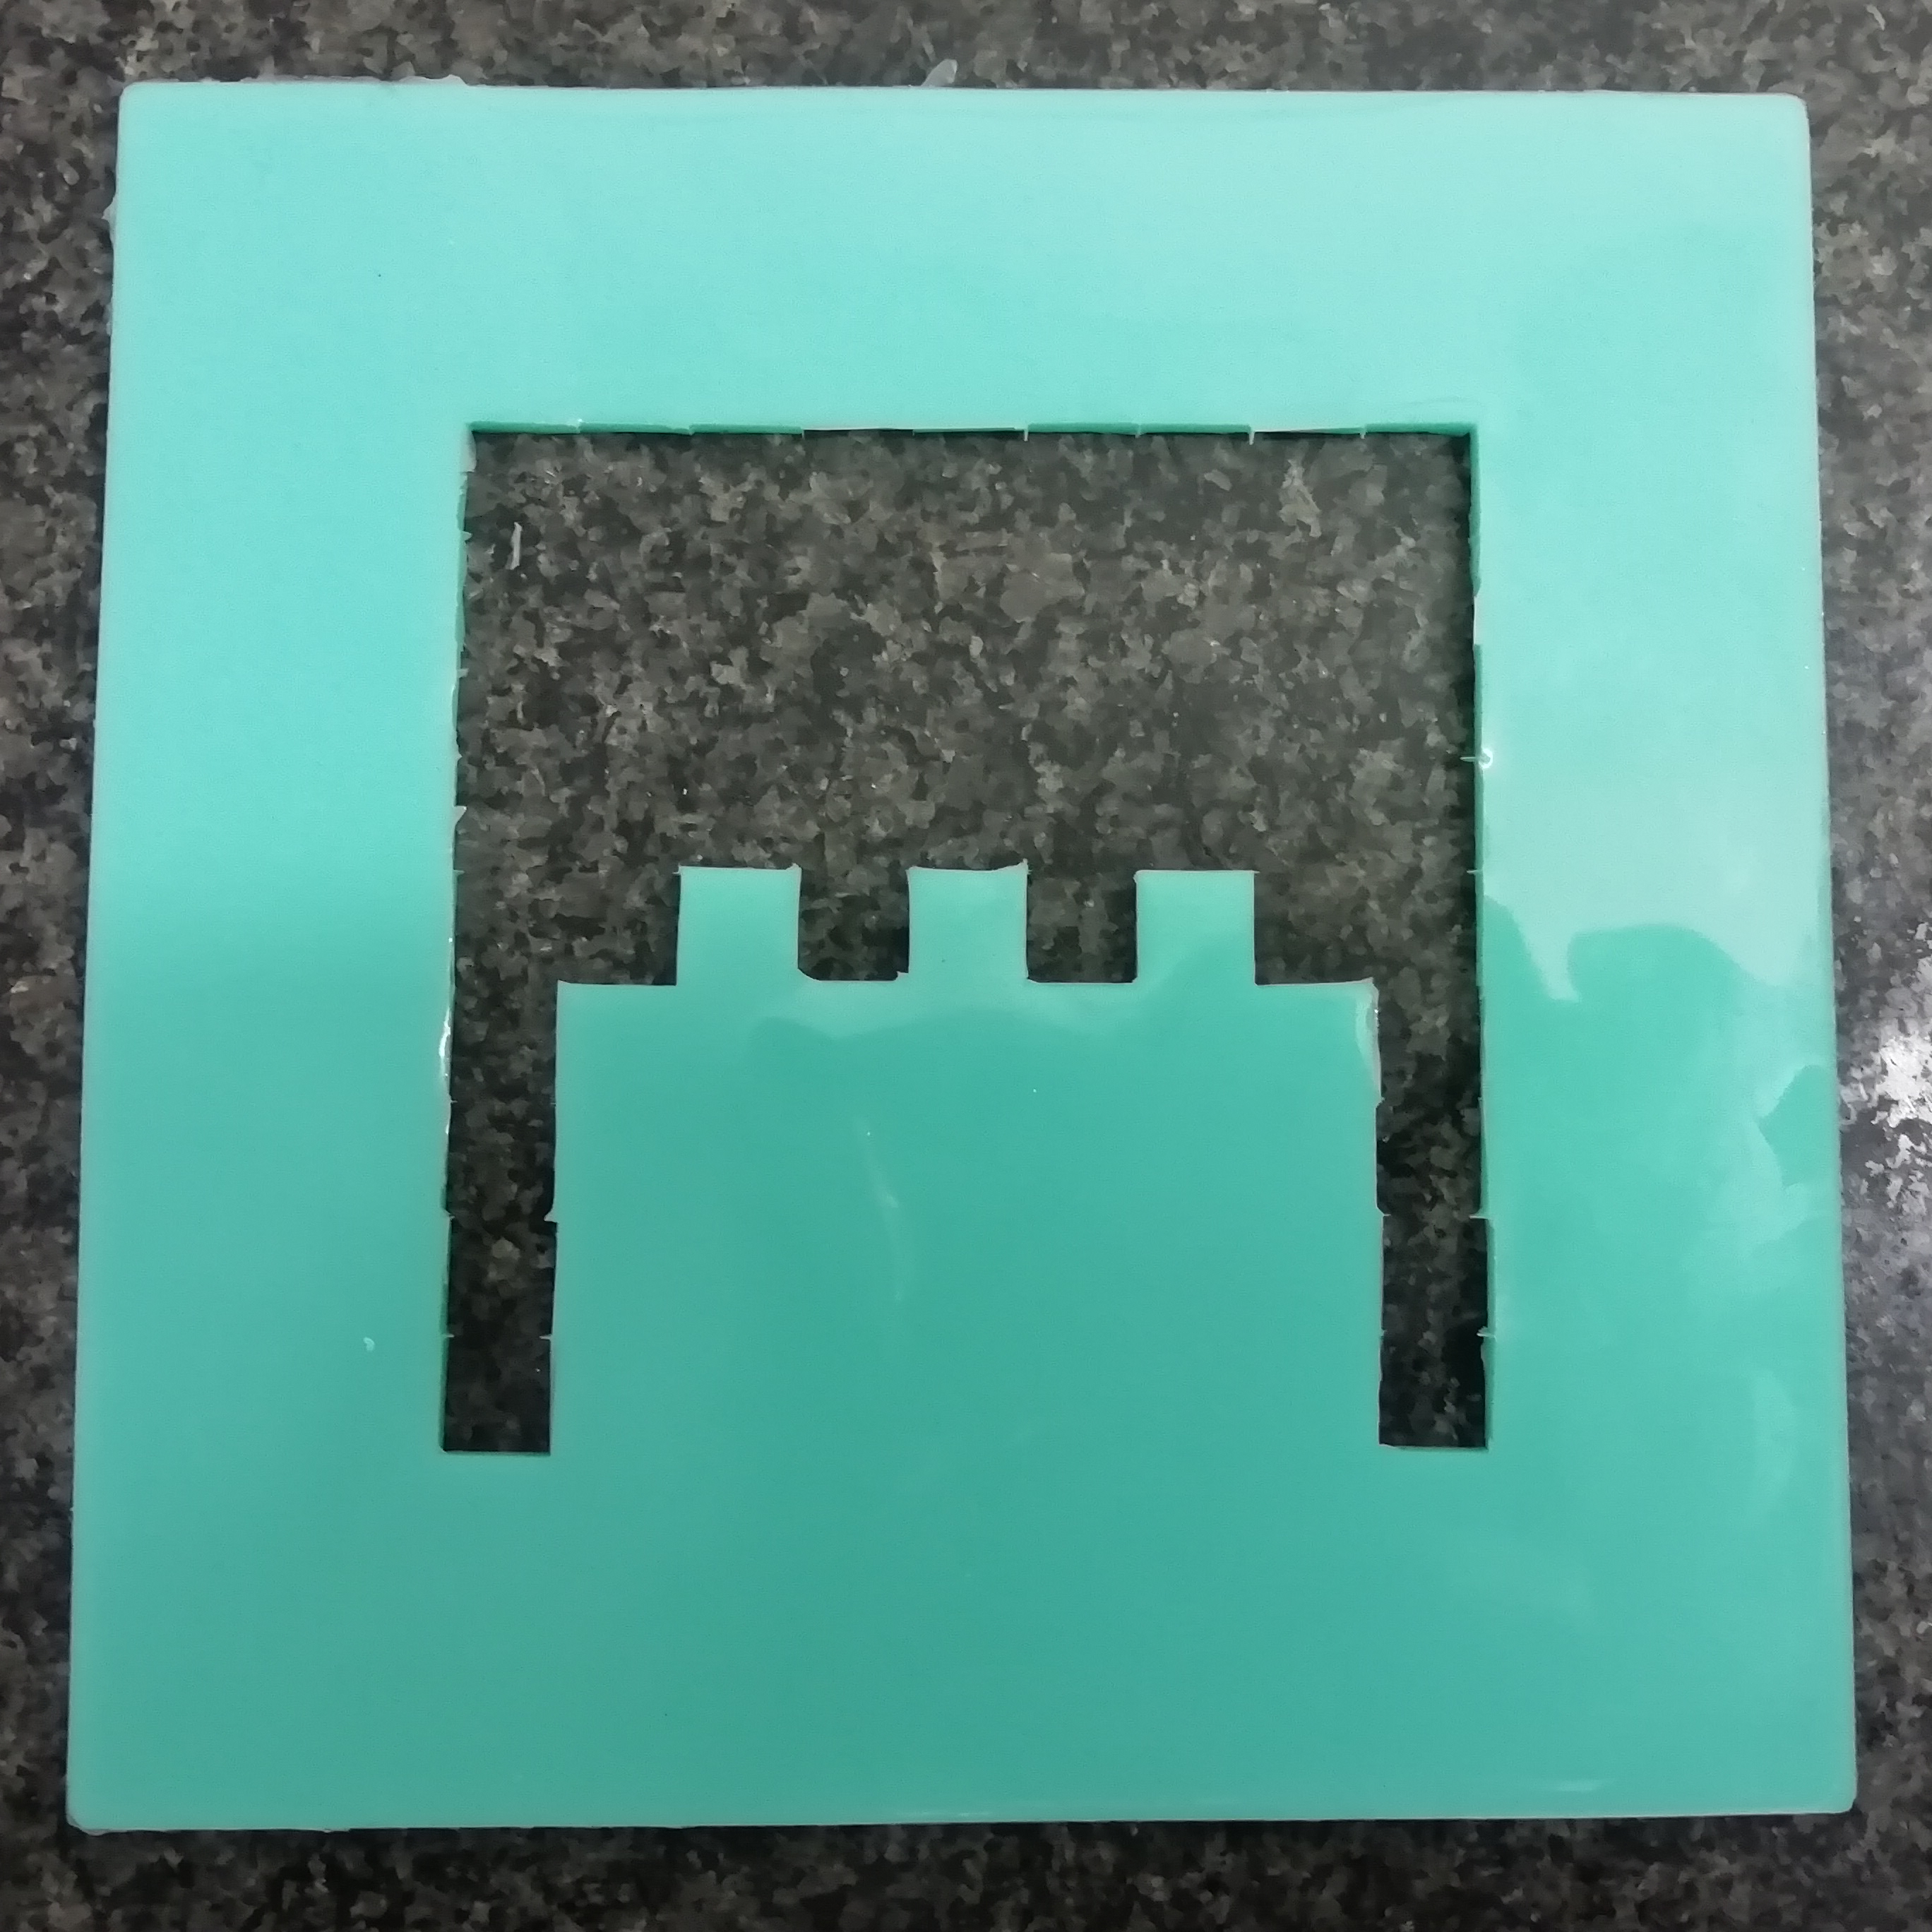
\includegraphics[width=\textwidth]{unit3mod.png}
		\caption{Physical validation model}
		\label{fig:unit3mod}
	\end{subfigure}
	\caption[FEM and physical models of unit 2]{grid\_57\_292a241d90d8d6b4753d110deca32360 FEM and physical validation models}
	\label{fig:unit3}
\end{figure}

Figure~\ref{fig:unit3def} shows comparisons between the FEM model and the physical model as the internal pressure is increased. Figure~\ref{fig:unit3over} illustrates an overlay of the FEM model deformation with the physical model's deformation. The FEM deformation is taken from step 2 of the simulation. The physical deformation is the final deformation.

\begin{figure}[H]
	\centering
	\begin{subfigure}[c]{\textwidth}
		\centering
		\includegraphics[width=\textwidth]{unit3deffem.png}
		\caption{FEM model deformation as internal pressure is increased. Steps 0-5 of the simulation are shown from left to right.}
	\end{subfigure}
	\hfill
	\begin{subfigure}[c]{\textwidth}
		\centering
		\includegraphics[width=\textwidth]{unit3defmod.png}
		\caption{Physical model deformation as internal pressure is increased}
	\end{subfigure}
	\caption[Comparison between FEM and physical models of unit 3]{Comparison between the deformation of the FEM model and physical model of grid\_50\_9a02e87afe77b71561f73745d87b35bd as the internal pressure is increased}
	\label{fig:unit3def}
\end{figure}

\begin{figure}[H]
	\centering
	\includegraphics[width=0.8\textwidth]{unit3defover.png}
	\caption[Physical model of unit 3 overlayed with FEM model]{grid\_50\_9a02e87afe77b71561f73745d87b35bd physical model overlayed with FEM model at step 2 of simulation}
	\label{fig:unit3over}
\end{figure}

\section{Results}

The FEM models were predictive of the behaviour of the physical units. The complex internal geometries behaved as expected, with minor differences. The unit outlines closely matched the predicted outlines. The FEM models may be considered accurate predictions of the physical models. The material models as obtained by \cite{Ellis2020} may be considered accurate as well.

\section{Issues, Discrepancies, and Solutions}

Some issues were encountered during model validation. Some were attempted to account for beforehand and some were unforeseen.

Mould cells were not manufactured exactly to tolerances. Several small and large mould cells were sanded by hand to remove rough edges or protrusions and to reduce their overall size. Several mould cells had uneven sides due to manufacturing or sanding. Material seeped into gaps between mould cells during casting. The bottom of the unit had excess material where the cast material had seeped into gaps. Excess material was carefully removed by hand but the surface was not perfectly smooth. Mould cells were laser cut. Having mould cells machined may be more costly but could result in higher quality mould cells.

Units placed between the perspex plates did not seal the internal area completely. Under higher pressures, air escaped by deforming the unit up or down against the perspex plates and escaping past the unit boundary. Clamps were applied to the edges of the perspex plates to seal the material better. Clamps may be a necessary permanent component of the experimental setup.

The silicon-based lubricant did not decrease the friction as much as was desired. A significant amount of force was required to move or deform the units even when only one side was in contact with the perspex. Clamping the sides of the perspex also increased the frictional resistance, as the unit was more compressed between the two plates. It is advisable to adjust the clamp strength accordingly so as to not clamp the unit too tightly.

The uneven side of the units in combination with the air leaking, clamping, and high friction is assumed to account for the discrepancies between the physical models and the FEM models.